\documentclass[10pt]{article}
\usepackage[margin=0.8in]{geometry}
\usepackage{amsmath,amssymb,amsfonts}
\usepackage{bm}
\usepackage{xcolor}
\usepackage{tikz}
\usetikzlibrary{positioning,arrows.meta,calc,fit,backgrounds,shapes.geometric}
\usepackage{caption}
\usepackage{enumitem}
\usepackage[hidelinks]{hyperref}
\usepackage{parskip}
\usepackage{titlesec}
\titlespacing*{\section}{0pt}{7pt}{2pt}
\titleformat{\section}{\normalfont\large\bfseries}{\thesection}{0.5em}{}
\captionsetup{font=footnotesize,labelfont=bf,skip=3pt}
\setlength{\parskip}{3.5pt}

\definecolor{phys}{HTML}{2C6E9B}\definecolor{agent}{HTML}{9B4DA0}
\definecolor{data}{HTML}{C9772B}\definecolor{ml}{HTML}{2E8B57}
\definecolor{softblue}{HTML}{E8F0F7}\definecolor{softpurple}{HTML}{F1E8F2}
\definecolor{softorange}{HTML}{FBEEDD}\definecolor{softgreen}{HTML}{E6F2EB}
\tikzset{
  proc/.style={rectangle,rounded corners=2pt,draw=phys!80,fill=softblue,align=center,inner sep=3pt,font=\scriptsize,minimum height=7mm},
  mlproc/.style={rectangle,rounded corners=2pt,draw=ml!80,fill=softgreen,align=center,inner sep=3pt,font=\scriptsize,minimum height=7mm},
  agproc/.style={rectangle,rounded corners=2pt,draw=agent!80,fill=softpurple,align=center,inner sep=3pt,font=\scriptsize,minimum height=7mm},
  art/.style={cylinder,shape border rotate=90,aspect=0.25,draw=data!85,fill=softorange,align=center,inner sep=2pt,font=\scriptsize\ttfamily,minimum height=7mm},
  flow/.style={-{Stealth[length=2mm]},thick,draw=black!65},
  fb/.style={-{Stealth[length=2mm]},thick,draw=agent!70,dashed},
  lbl/.style={font=\tiny\itshape,text=black!55},
}

\newcommand{\bx}{\mathbf{x}}\newcommand{\bz}{\mathbf{z}}\newcommand{\by}{\mathbf{y}}
\newcommand{\bc}{\mathbf{c}}\newcommand{\bK}{\mathbf{K}}\newcommand{\bV}{\mathbf{V}}
\newcommand{\bI}{\mathbf{I}}\newcommand{\bmu}{\bm{\mu}}
\newcommand{\Ffwd}{\mathcal{F}}\newcommand{\Fhat}{\hat{\mathcal{F}}}
\newcommand{\R}{\mathbb{R}}\newcommand{\E}{\mathbb{E}}\newcommand{\GP}{\mathcal{GP}}
\newcommand{\indic}{\mathbb{1}}
\DeclareMathOperator{\Var}{Var}\DeclareMathOperator{\RMSE}{RMSE}
\DeclareMathOperator*{\argmin}{arg\,min}\DeclareMathOperator*{\argmax}{arg\,max}
\newcommand{\Lstar}{\Delta^{\!*}}

\pagestyle{empty}
\begin{document}

\begin{center}
{\Large\bfseries Autotokamak: Fast Learned Surrogates for the Grad--Shafranov Equilibrium}\\[2pt]
{\normalsize A plain-language two-page summary}
\end{center}
\vspace{-2pt}

\noindent\textit{In one sentence:} we train a machine-learning model that reproduces a slow
physics simulation of a fusion plasma almost instantly, and we use an AI agent to run the whole
data-collection-and-training process automatically, spending the expensive simulations only where
the model still makes mistakes.

\section{The problem: a simulation that is accurate but slow}
A \textbf{tokamak} is a doughnut-shaped device that confines hot plasma with magnetic fields for
fusion energy. To design or control one, engineers must know the plasma's \emph{equilibrium}: the
shape of the nested magnetic surfaces that hold it in place. Mathematically the equilibrium is a
2-D field $\psi(R,Z)$ --- think of it as a heat-map image over a cross-section of the doughnut ---
that solves a nonlinear partial differential equation, the \textbf{Grad--Shafranov (GS) equation}
$\ \Lstar\psi = -\mu_0 R^2 p'(\psi) - F(\psi)F'(\psi)$. The industry-standard solver (TokaMaker,
from the OpenFUSION Toolkit) computes $\psi$ with the finite-element method: accurate, but it takes
seconds to minutes for a \emph{single} design. Anyone who wants to scan thousands of designs, or
steer a plasma in real time, cannot afford that.

Our idea is to \emph{learn a fast stand-in for the slow solver}. We regard the solver as a function
that takes five design numbers and returns the flux image:
$$
\Ffwd:\ \bx=(\underbrace{R_0,\,a,\,\kappa,\,\delta}_{\text{plasma shape}},\ \underbrace{I_p}_{\text{current}})\ \in\R^5\ \longmapsto\ \psi(R,Z)\ \ (\text{a } 96\times64 \text{ image}).
$$
The goal is a learned approximation $\Fhat\approx\Ffwd$ that runs in milliseconds. Because every
training example costs one expensive solve, a second goal is to \emph{choose those solves wisely}.
The system runs in three stages (Fig.~\ref{fig:flow}): (1)~generate a starting dataset, (2)~fit the
fast model, and (3)~an outer ``meta-loop'' that repeatedly improves the data and the model, with an
AI agent deciding what to do next.

\begin{figure}[h]
\centering
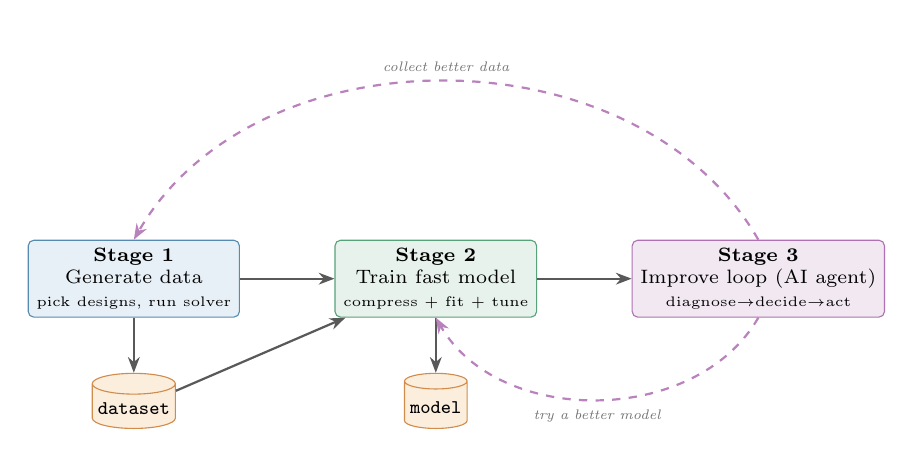
\begin{tikzpicture}[node distance=8mm]
  \node[proc] (p1) {\textbf{Stage 1}\\Generate data\\{\tiny pick designs, run solver}};
  \node[mlproc,right=12mm of p1] (p2) {\textbf{Stage 2}\\Train fast model\\{\tiny compress + fit + tune}};
  \node[agproc,right=12mm of p2] (p3) {\textbf{Stage 3}\\Improve loop (AI agent)\\{\tiny diagnose$\to$decide$\to$act}};
  \node[art,below=7mm of p1] (a1) {dataset};
  \node[art,below=7mm of p2] (a2) {model};
  \draw[flow](p1)--(p2);\draw[flow](p2)--(p3);\draw[flow](p1)--(a1);\draw[flow](p2)--(a2);\draw[flow](a1)--(p2);
  \draw[fb] (p3.north) to[out=120,in=60] node[lbl,above]{collect better data} (p1.north);
  \draw[fb] (p3.south) to[out=240,in=300] node[lbl,below]{try a better model} (p2.south);
\end{tikzpicture}
\caption{The three stages. Solid arrows are the forward pipeline; dashed arrows are the Stage-3
decisions that loop back to gather better data or search for a better model. Only those high-level
decisions are made by the AI; every calculation is ordinary, reproducible code.}
\label{fig:flow}
\end{figure}
\vspace{-6pt}

\section{The fast model: compress the image, then predict a few numbers}
Predicting all $96\times64 = 6144$ pixels of the flux image directly would be wasteful, because the
images are highly repetitive --- across many designs they are near-copies of a few basic patterns.
We exploit this with \textbf{Principal Component Analysis (PCA)}, a standard technique that finds
the handful of ``building-block'' images $\bV_k$ whose weighted sums reconstruct any field in the
dataset. Each flux image is then summarized by just $k$ numbers (its \emph{coefficients}, about 8
suffice here). Predicting the image reduces to predicting those few numbers and re-expanding:
$$
\boxed{\ \Fhat(\bx)=\bar\by+\textstyle\sum_{j=1}^{k} g_j(\bx)\,\bV_{k,j}\ }
\qquad\text{(mean image $+$ a weighted sum of building blocks).}
$$
Each coefficient $g_j$ is predicted from the five design numbers by a small regressor. Our main
choice is a \textbf{Gaussian Process (GP)} --- a probabilistic regressor that is accurate with few
training points and, crucially, also reports \emph{how confident} it is. Its prediction is a
weighted average of the solved examples nearby, and its uncertainty grows as you move away from the
data:
$$
\underbrace{\mu_j(\bx_\star)=\mathbf{k}_\star^\top(\bK+\alpha\bI)^{-1}\bc^{(j)}}_{\text{prediction}}
\qquad
\underbrace{\sigma_j^2(\bx_\star)=k(\bx_\star,\bx_\star)-\mathbf{k}_\star^\top(\bK+\alpha\bI)^{-1}\mathbf{k}_\star}_{\text{uncertainty}} .
$$
(Three simpler regressors --- kernel ridge, polynomial ridge, and a small neural network --- are
also available.) Each model has settings (``hyperparameters''); we tune them automatically with
\textbf{Optuna}, a Bayesian optimizer, minimizing the error measured by cross-validation (train on
part of the data, test on the held-out part). The tuned model is only kept if it beats a trivial
baseline --- predicting the \emph{average} image every time --- reported as a percent error
reduction.

\section{Spending simulations wisely: sample where the model is weak}
A model is rarely equally good everywhere; it is usually accurate in well-sampled regions and poor
in a few corners of the design space. Randomly picking the next simulations wastes most of them on
regions the model already handles. Instead we \emph{measure where the current model is wrong} (its
error on held-out examples), train a second small GP to predict that error across the whole design
space, and then choose new simulation points by scoring each candidate design with an
\textbf{Upper Confidence Bound (UCB)}:
$$
\boxed{\ \text{score}(\bx)=\underbrace{\mu_g(\bx)}_{\substack{\text{predicted}\\\text{error (exploit)}}}\ +\ \beta\underbrace{\sigma_g(\bx)}_{\substack{\text{uncertainty}\\\text{(explore)}}}\ +\ \underbrace{\log P_{\text{feasible}}(\bx)}_{\substack{\text{avoid designs the}\\\text{solver can't handle}}}\ }
$$
In words: prefer designs where the model is \emph{predicted to be bad}, or where we simply
\emph{don't yet know} (the tunable weight $\beta$ balances the two), while avoiding extreme shapes
that make the physics solver fail --- a failure probability we also learn from past successes and
failures. We select a spread-out \emph{batch} of such designs (not many copies of the single worst
point), run the solver on them, add the results to the dataset, and retrain. To prove this helps,
we score every model on a fixed, held-out test set that covers the full design space, broken down
\emph{region by region}, and we compare against a control that just adds random designs on the same
simulation budget.

\section{The AI agent that runs the whole loop}
Stage 3 wraps all of the above in an automated decision loop. Each round, ordinary code produces a
\emph{diagnosis} of the current state (how good is the model, where is it weak, how many solves
failed), and a large language model (LLM) reads it and picks one clearly-defined next action:
$$u\in\{\ \texttt{collect more data},\ \ \texttt{collect smarter data},\ \ \texttt{re-tune the model},\ \ \texttt{stop}\ \}.$$
The action is validated and then carried out by ordinary code. This is the key design choice:
\textbf{the AI only makes high-level strategic decisions; every number --- the physics, the model
fitting, the error scoring --- is computed by deterministic, reproducible code}, so the results are
trustworthy and repeatable. Finally, we grade each complete run with a single score that rewards
accuracy, steady improvement, not wasting budget, and stopping decisively; the agent's
decision-making is then automatically improved against that score.

\vspace{3pt}
\noindent\textbf{Why it matters.} Autotokamak delivers a millisecond replacement for a
minutes-long plasma-equilibrium simulation, \emph{and} an automated pipeline that decides for
itself where to spend expensive simulations and when to stop --- combining a machine-learning
contribution (the fast surrogate) with an automation contribution (the self-directed agentic loop).

\end{document}
